Describe your method in detail and with great clarity, distinguishing it from
other works (if it is indeed a novel idea). It is very important to clearly
motivate your method.

Describe the results of your method here in this chapter.

All computational work for this thesis was performed in \textit{MATLAB vR2023a}
unless stated otherwise.

\section{Datasets}

Crous~\cite{crous2019polyphonic} has some data on Xeno-canto.

Since all the models described in Section~\ref{sec:classification} are trained
in a supervised learning fashion, this requires a dataset of labelled training
examples. The website xeno-canto.org (XC) houses the largest and most
comprehensive publicly available collection of birdsong samples in the world. It
has made an enormous impact in the field birdsong recognition since its
inception in 2005 and has been source of the datasets for the annual BirdCLEF
challenge since 2014~\cite{vellinga2015xeno}. All samples available on XC are
labelled with the bird species and contain rich metadata, such as the time and
location of the recording. Importantly, all samples have a crowd-sourced rating
from A --- E which signifies how clear the recording sample is, where A denotes
samples with the highest quality and clarity. This is especially important
should we wish to experiment with different signal-to-noise ratios (SNR) as the
noise can be manually added to a clean recording at precise SNR levels. 

Due to its scale and reputation in the birdsong classification community, all
samples used in this thesis have been downloaded from the XC repository. All
samples downloaded have an A rating and have been labelled as a `song' rather
than a `call'. The samples are stored in a directory labelled according to the
first three letter of species' binomial name. For example, samples from the
common blackbird (\textit{Turdus merula}) are stored in a directory called
`TURMER'. This directory name acts as a label for training and test samples.

In this work we are mostly concerned with testing relative improvements in model
performance after tuning various components, such as novel feature
representations. To this end, we select the most simple form of classification
experiment: binary classification. The two bird classes selected for all
experiments herein are the common blackbird and the common nightingale
(\textit{Luscinia megarhynchos}) due to the two birds' vocalizations being
acoustically similar and hence more difficult to distinguish resulting in more
variable accuracy results, and the author's personal preference.

\section{Pre-processing}

Some recordings available on XC are recorded in stereo sound, so in order to
reduce dimensionality without losing too much information, all recordings are
first converted to mono by taking a mean average of both channels. Leading and
trailing sections of background noise are then stripped from the recording using
the \textit{detectSpeech} function provided by \textit{MATLAB}. This function
uses a thresholding algorithm to detect onset and offset indices of
speech~\cite{giannakopoulos2009method}. The function works for birdsong since
birdsong frequencies reside in a similar range to that of human speech. The
function accepts various arguments to determine properties such as window length
and threshold value, but from initial experiments, the function was shown to
work well with birdsong with the defaults, see figure~\ref{fig:detected_speech}.
The detected onset and offset of birdsong allows for the leading and trailing
bits of background noise to be removed from the recording, thus reducing
unnecessary computational time in segmenting the audio.

\begin{figure}[ht]
  \centering
  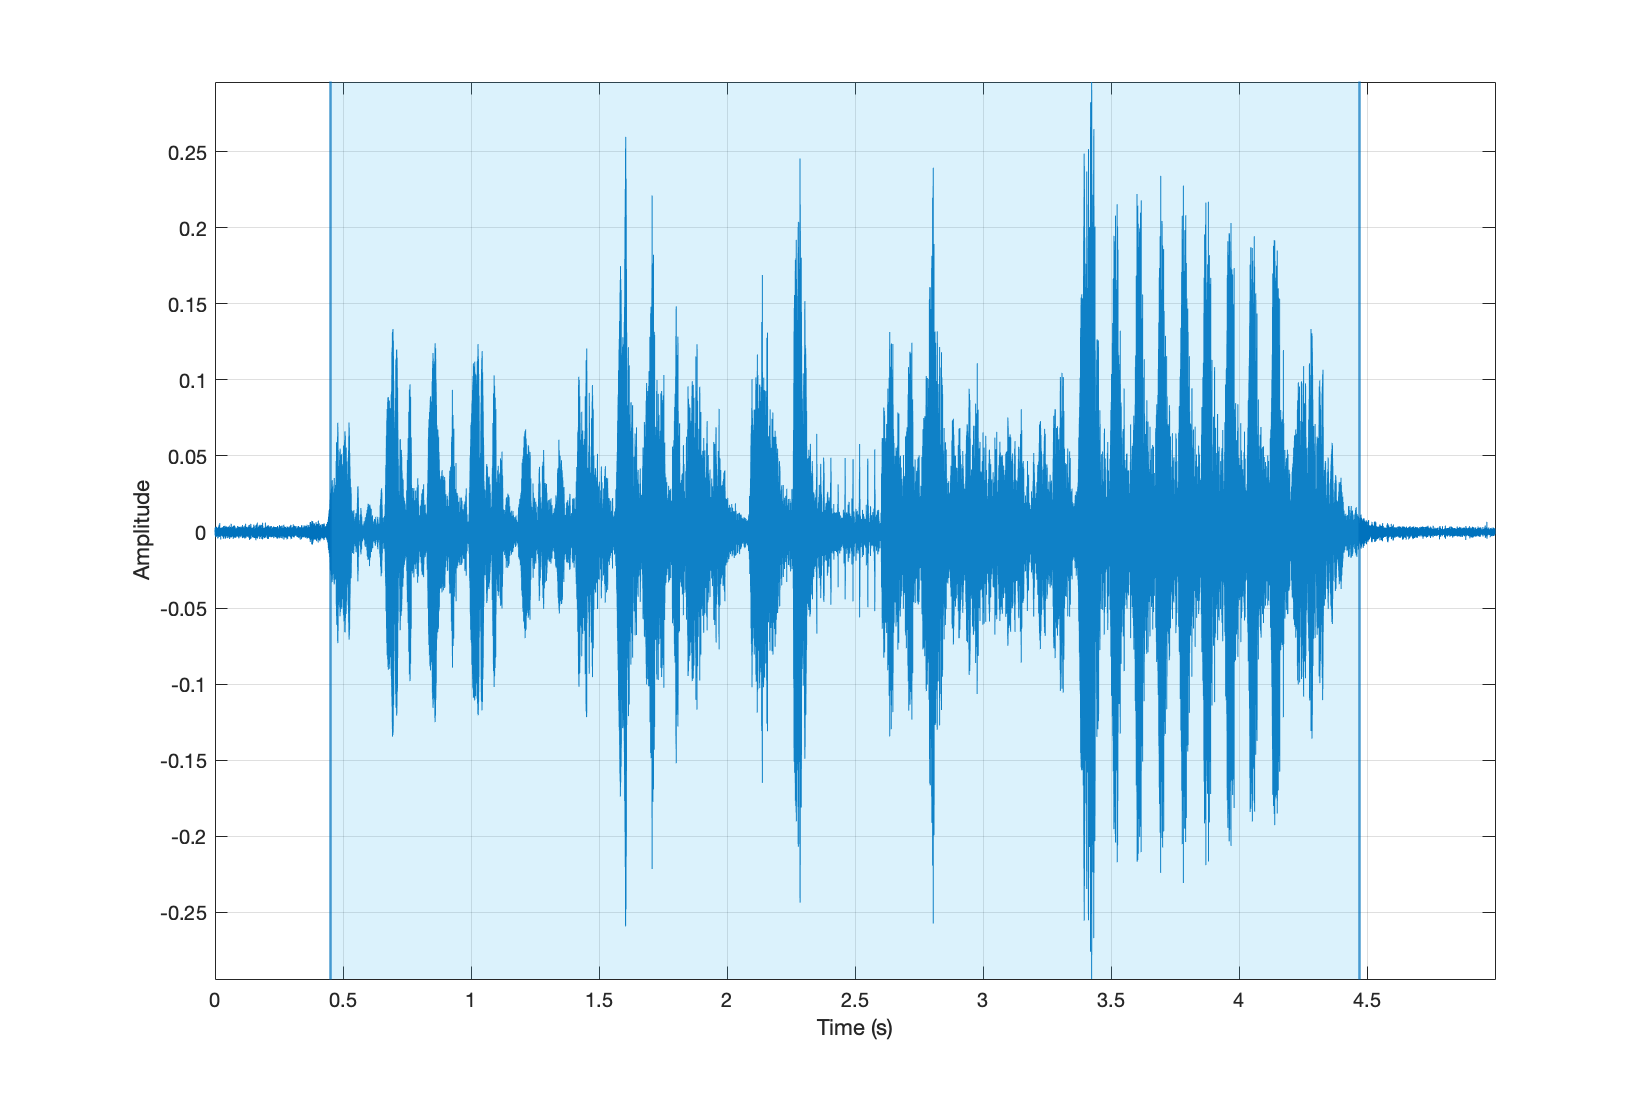
\includegraphics[width=\textwidth]{figures/detected_speech.png}
  \caption{Output of the \textit{detectSpeech} function for a recording of
  birdsong from a Eurasian wren. The highlighted section shows where the
algorithm has detected `speech', or in this case,
birdsong.}\label{fig:detected_speech}
\end{figure}

A highpass filter is then applied to the recording with a passband frequency of
450Hz. This value was chosen as most birdsong sits in the range of 1KHz ---
10Khz, and so lower frequencies can be attributed to background noise and
therefore their removal should reduce noise in the system without losing
important information. The reason why frequencies above 10Khz are note removed
is that, as can be seen from figure~\ref{fig:wren_call_song_spectrogram}, birds
typically produce higher frequency harmonics when vocalizing, shown as vertical
bands moving upwards from where syllables are located on the spectrogram. These
harmonics may capture useful information for the learning algorithm to utilise.

After these pre-processing steps have been taken, the audio is ready for
syllable segmentation.

\section{Segmentation}

Recordings downloaded from XC were also chosen based on their length. Recordings
of duration 40 seconds to 120 seconds were preferred since they were likely to
be long enough to include enough variety of vocalizations from one individual
bird, but not too long so as to take up too much space on disk. In this thesis
it was preferred to have fewer samples from more individual as opposed to more
samples from fewer individuals for each species. The intention of this was to
introduce more variation in the training samples for each class, especially when
considering that many birds of the same species but residing in different
locations have demonstrated subtle variations in vocalizations, known as
dialects~\cite{baker1985biology}. As a general rule of thumb, a target of
roughly 50 training samples per individual was aimed for in this thesis.

This leads to the question of how to generate samples. In the literature there
seem to be two main ways of segmenting recordings into samples to be used for
training. The first is segmenting a recording into overlapping segments of a
certain length, typically in the range of 4 --- 11 seconds
(\cite{yan2021birdsong},~\cite{crous2019polyphonic}). This has the advantage
that all samples will be of fixed length and that the segmentation algorithm is
very simple. However, it will likely mean that some samples will contain only
background noise which, if used for training, will introduce noise into the
system. These noise samples therefore may need to be removed, either
manually~\cite{yan2021birdsong} or using an
algorithm~\cite{narasimhan2017simultaneous}. The other method involves
segmenting the recording into syllables
(\cite{fagerlund2007bird},~\cite{ramashini2022robust}). This has the advantage
that all training samples are likely to contain little or no noise. However the
samples will be of variable length, so steps will be needed to be taken in order
to compare the samples, such as adding padding or more advanced techniques like
dynamic time warping~\cite{somervuo2006parametric}. Syllable segmentation also
has the enticing prospect of being able to identify a bird species from a very
short sample. This could be useful in situations where a recording is mostly
corrupted by background noise but has a few small segments of clear birdsong.

In this work we attempt to combine the benefits of both approaches by first
segmenting a recording to retrieve the syllables using a process described in
Section~\ref{ssec:syllable_seg}. Then, for each syllable, the
following syllables are appended until a fixed sample length is reached. If a
syllable is added which pushes the sample length over the limit, then the sample
is trimmed at the fixed length. This approach is motivated by Somervuo et al.'s
work~\cite{somervuo2006parametric} in showing that training and classifying
using single syllables returns suboptimal results, whereas using sequences of
syllables gives much improved accuracy. Of course there is a tradeoff here
between training with longer sequences, and hence more information, versus
increased computational demand to perform training. With this tradeoff in mind,
a fixed length of 13230 is chosen. <Add figure of histogram here showing lengths
of syllables>. Typical syllable length is X, and so the fixed length should
contain roughly Y syllables. This approach ensures the influence of background
noise is kept to a minimum, while still maintaining information related to the
temporal evolution of a particular birdsong.

\subsection{Energy based syllable segmentation}\label{ssec:syllable_seg}

This algorithm was first proposed by Fagerlund~\cite{fagerlund2004automatic}
and has been used in various research papers since
(\cite{somervuo2006parametric},~\cite{ramashini2022robust}). Note that Fagerlund
proposed two different segmentation methods in the paper. In this thesis we use
the energy based segmentation method as it's relatively
simple to implement and its performance can be superior to the other method
proposed. The algorithm is computed in the following 3 phases:

\begin{enumerate}

  \item Determine the onsets and offsets of syllable candidates. Special
    attention has to be paid to the border effect~\cite{li2001classification},
    whereby the energy envelope near onsets and offsets fluctuates around a
    threshold.

  \item Syllable candidates that are within a certain temporal distance with
    each other are merged into one. The initial separation of candidates can
    likely be attributed to the border effect, and so the candidates can be
    thought of as originating from one syllable in reality.

  \item Syllable candidates that are shorter than a minimum threshold are
    removed. These candidates are often caused by random fluctuations in the
    signal energy and are unrelated to bird vocalizations.

\end{enumerate}

\subsubsection{Onset/offset detection}

The first phase considers the energy of an input signal. The energy envelope is
the key variable to use in determining the onset and offset of a syllable. The
general idea is that when the energy increases past a threshold, this marks the
start of a syllable candidate and when the energy then falls below the same
threshold, this marks the end of a syllable candidate. To calculate the energy
envelope, the recording is divided into overlapping frames.
Fagerlund~\cite{fagerlund2004automatic} recommends a frame size of 128 samples
and an overlap of 50\%. This corresponds to a frame length of roughly 3ms. Since
distance between syllables can be as short as 20ms, the frame size needs to be
small enough so that there are at least a few frames between candidates to be
able to efficiently discriminate between syllables.

Frames are first windowed using a Hanning window. The energy $E_i$ in the
decibel scale for frame $i$ is calculated as
\begin{equation}
  E_i = 10 \log_{10} \sum_{j=1}^{K} x{(i)}_{j}^2
\end{equation}
where $x{(i)}_j$ is the $j^{\text{th}}$ input signal sample value in the
$i^{\text{th}}$ frame and $K$ is the total number of samples in each frame, in
this case 128. The maximum energy of the entire signal is normalized to 0dB.
The initial noise level estimate is set to be equal to global minimum value of
the energy envelope and the threshold for the onset and offset detection is set
to half the noise estimate. The flow diagram for onset and offset detection can
be seen in figure <figure of flow chart>. In essence, the algorithm moves
through each frame and computes whether the frame should be assigned to a
syllable or not. The noise estimate is updated as the average energy of frames
already processed by the algorithm that are not assigned to a syllable.

\subsubsection{Merging syllable candidates}

The algorithm may produce syllable candidates that are very temporally close
together. This may be from the bird producing short bursts of pulses that
constitute the same syllable, or it may be from the border effect. In both cases
the candidates can be considered as belonging to the same syllable and so can be
safely merged together. Candidates that are less than 15ms apart are selected
for merging~\cite{fagerlund2004automatic}.
